\documentclass[landscape,final,a0paper,fontscale=0.285]{baposter}

\usepackage{calc}
\usepackage{graphicx}
\usepackage{amsmath}
\usepackage{amssymb}
\usepackage{relsize}
\usepackage{multirow}
\usepackage{rotating}
\usepackage{bm}
\usepackage{url}

\usepackage{graphicx}
\usepackage{multicol}

%\usepackage{times}
%\usepackage{helvet}
%\usepackage{bookman}
\usepackage{palatino}
%\usepackage{arial}

\newcommand{\captionfont}{\footnotesize}

\graphicspath{{images/}{../images/}}
\usetikzlibrary{calc}

\newcommand{\SET}[1]  {\ensuremath{\mathcal{#1}}}
\newcommand{\MAT}[1]  {\ensuremath{\boldsymbol{#1}}}
\newcommand{\VEC}[1]  {\ensuremath{\boldsymbol{#1}}}
\newcommand{\Video}{\SET{V}}
\newcommand{\video}{\VEC{f}}
\newcommand{\track}{x}
\newcommand{\Track}{\SET T}
\newcommand{\LMs}{\SET L}
\newcommand{\lm}{l}
\newcommand{\PosE}{\SET P}
\newcommand{\posE}{\VEC p}
\newcommand{\negE}{\VEC n}
\newcommand{\NegE}{\SET N}
\newcommand{\Occluded}{\SET O}
\newcommand{\occluded}{o}

%%%%%%%%%%%%%%%%%%%%%%%%%%%%%%%%%%%%%%%%%%%%%%%%%%%%%%%%%%%%%%%%%%%%%%%%%%%%%%%%
% Multicol Settings
%%%%%%%%%%%%%%%%%%%%%%%%%%%%%%%%%%%%%%%%%%%%%%%%%%%%%%%%%%%%%%%%%%%%%%%%%%%%%%%%
\setlength{\columnsep}{1.5em}
\setlength{\columnseprule}{0mm}

\newcommand{\compresslist}{%
\setlength{\itemsep}{1pt}%
\setlength{\parskip}{0pt}%
\setlength{\parsep}{0pt}%
}

\begin{document}

% Define some colors

\definecolor{lightblue}{cmyk}{0.83,0.24,0,0.12}
\definecolor{lightblue}{rgb}{.1,.43,.14}

\begin{poster}%
  % Poster Options
  {
  % Show grid to help with alignment
  grid=false,
  % Column spacing
  colspacing=1em,
  % Color style
  bgColorOne=white,
  bgColorTwo=white,
  borderColor=black,
  headerColorOne=lightblue,
  headerColorTwo=lightblue,
  headerFontColor=white,
  boxColorOne=white,
  boxColorTwo=lightblue,
  % Format of textbox
  textborder=roundedleft,
  % Format of text header
  eyecatcher=true,
  headerborder=closed,
  headerheight=0.1\textheight,
  textfont=\sc, %An example of changing the text font
  headershape=roundedright,
  headershade=shadelr,
  headerfont=\Large\bf\textsc, %Sans Serif
  textfont={\setlength{\parindent}{1.5em}},
  boxshade=plain,
%  background=shade-tb,
  background=plain,
  linewidth=2pt
  }
  % Eye Catcher
  {
\includegraphics[height=5em]{img/Clarkson}} 
  % Title
  {\bf\textsc{Dynamic Model for Balancing\\ Deer Population and Insurance Fund}\vspace{0.5em}}
  % Authors
  {\textsc{Kelly Black, Candace Liu, Elizabeth Sweeney, Lindong Zhou}}
  % University logo
  {% The makebox allows the title to flow into the logo, this is a hack because of the L shaped logo.
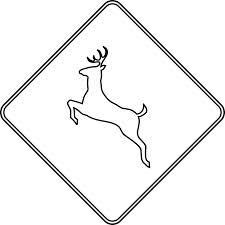
\includegraphics[height=6.0em]{img/deeroutline}
  }


%%%%%%%%%%%%%%%%%%%%%%%%%%%%%%%%%%%%%%%%%%%%%%%%%%%%%%%%%%%%%%%%%%%%%%%%%%%%%%
  \headerbox{Background}{name=definition,column=0,row=0}{

In the United States between July 1, 2011 and June 30, 2012
\begin{itemize}
	\item 1.23 million deer-vehicle collisions occured
	\item Costs are more than \$ 4 billion in vehicle damage
	\item The average claim for deer-vehicle collisions was \$3,305 per accident.
	\item The Insurance Institute for Highway Safety (IIHS) noted that deer-vehicle collisions in the U.S. cause about 200 fatalities annually. 
\end{itemize}
\emph{(State Farm, Insurance Journal)} \vspace*{.5cm} \\ 
For an insurance company to handle the claims of deer-vehicle collisions, it is important to understand the basics of how an insurance company manages their funds. Insurance companies \vspace{.1cm}
\begin{itemize}
	\item Invest in low risk government bonds
	\item Receive premiums from customers
	\item Claims are based on accidents \vspace{.1cm}
\end{itemize}
We examine the interaction of deer populations and the bond fun. \vspace{.5cm}
}

%%%%%%%%%%%%%%%%%%%%%%%%%%%%%%%%%%%%%%%%%%%%%%%%%%%%%%%%%%%%%%%%%%%%%%%%%%%%%%
  \headerbox{Logistic}{name=simple,column=1,row=0}{
To establish the logistic equation for the deer population, we assume that there are low predation rates, and interactions with people represent the greatest threats to white-tailed deer, which is \vspace*{-.2cm}
\begin{eqnarray} \label{eqn:detmodel}
	\frac{dx}{dt} &=& rx \left(1-\frac{x}{f}\right)-hx,
\end{eqnarray}\vspace*{-.6cm}
\begin{itemize}
	\item $f$ - carrying capacity \vspace*{-.3cm}
	\item $r$ - growth rate \vspace*{-.3cm}
	\item $h$ - harvest rate.
\end{itemize} \vspace*{-.2cm}
By combining terms, (\ref{eqn:detmodel}) can be rewritten as  \vspace*{-.3cm}
\begin{eqnarray}\label{eqn:scaled}
	\frac{dx}{dt} &=& \tilde{r} x\left( 1-\frac{x}{ \tilde{f} } \right)
\end{eqnarray}  \vspace*{-.1cm} where $\tilde{r}=r-h$ and $\tilde{f}=\frac{r-h}{r}f.$
}

%%%%%%%%%%%%%%%%%%%%%%%%%%%%%%%%%%%%%%%%%%%%%%%%%%%%%%%%%%%%%%%%%%%%%%%%%%%%%%
%  \headerbox{Limitations of $R_{0}$}{name=limitations,column=0,above=bottom}{
 % }

%%%%%%%%%%%%%%%%%%%%%%%%%%%%%%%%%%%%%%%%%%%%%%%%%%%%%%%%%%%%%%%%%%%%%%%%%%%%%%
  \headerbox{Approximations}{name=Zombie,column=1,span=1,above=bottom}{
To analyze the stochastic model, we must approximate the deer population \vspace*{-.4cm}
  \begin{eqnarray*}
    X(t) & = & X(a) + \int^t_a f(X) \, ds + \int^t_a g(X) \, dW(s). \vspace*{-.5cm}
  \end{eqnarray*}
Milstein method has an error of order $O(\Delta t^{1.5})$: \vspace*{-.3cm}
 \begin{eqnarray*}
   \hspace*{-.05cm} X_{j} &=& X_{j-1} + \triangle tf(X_{j-1}) \\
    && + g(X_{j-1})(W(\tau_{j})-W(\tau_{j-1}) \\
    && + .5 g(X_{j-1})g'(X_{j-1}) \\
    && ((W(\tau_{j})-W(\tau_{j-1}))^{2}-\triangle t)\\
    j &=& 1,2,... ,L 
  \end{eqnarray*}
 }

%%%%%%%%%%%%%%%%%%%%%%%%%%%%%%%%%%%%%%%%%%%%%%%%%%%%%%%%%%%%%%%%%%%%%%%%%%%%%%
\headerbox{Simulation Results}{name=graphs,column=2,span=2}{
\centering
\hspace*{-.5cm}
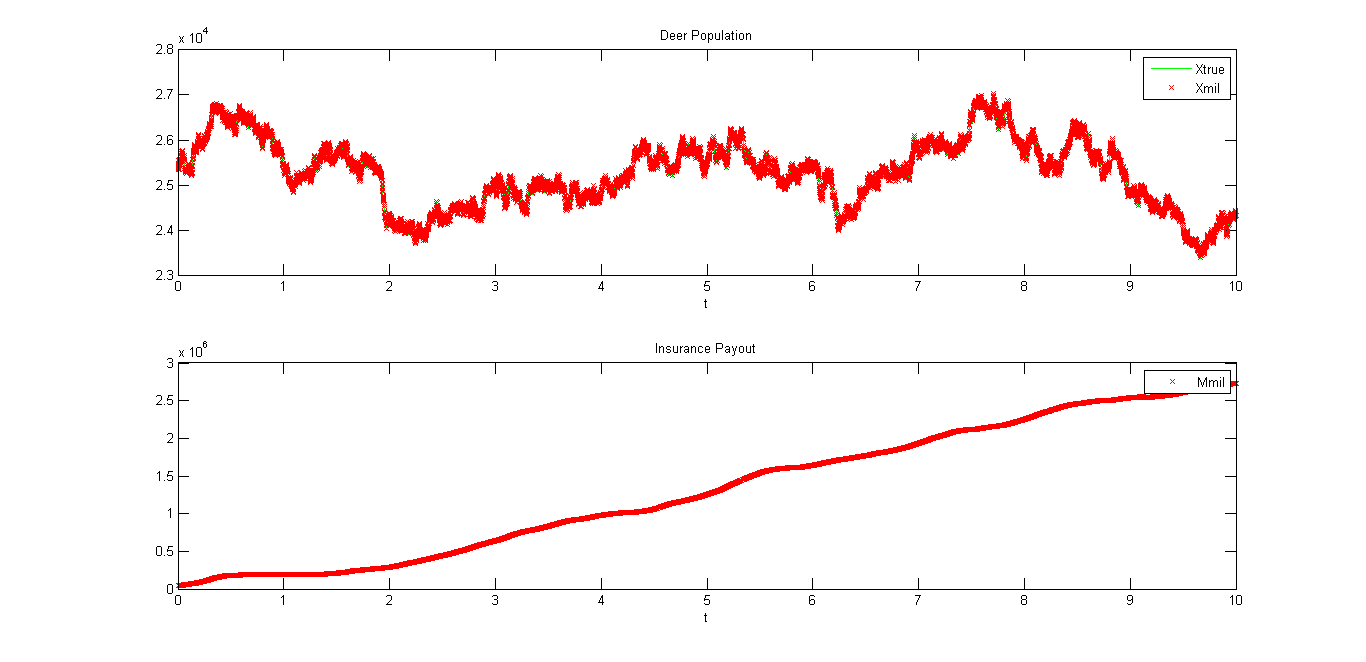
\includegraphics[height=4.2cm]{img/deerins}  
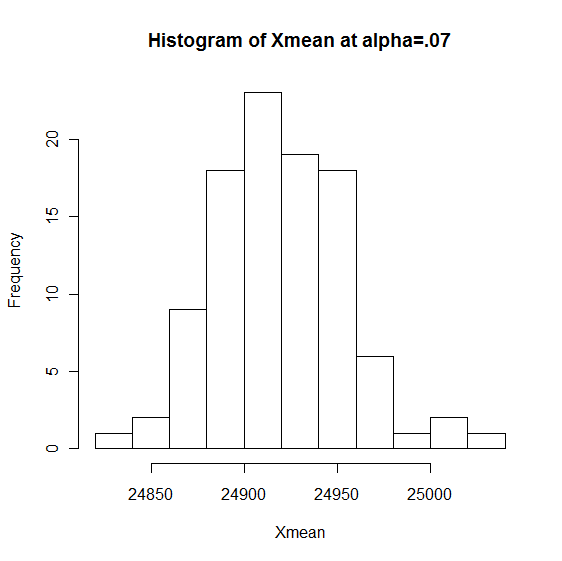
\includegraphics[width=4cm]{img/hist1000_xmean_alpha07} \\
One Run with $\alpha=.05$, $\gamma=.05$, $P=230000$ and Histogram of the Mean Population with 1000 iterations\\
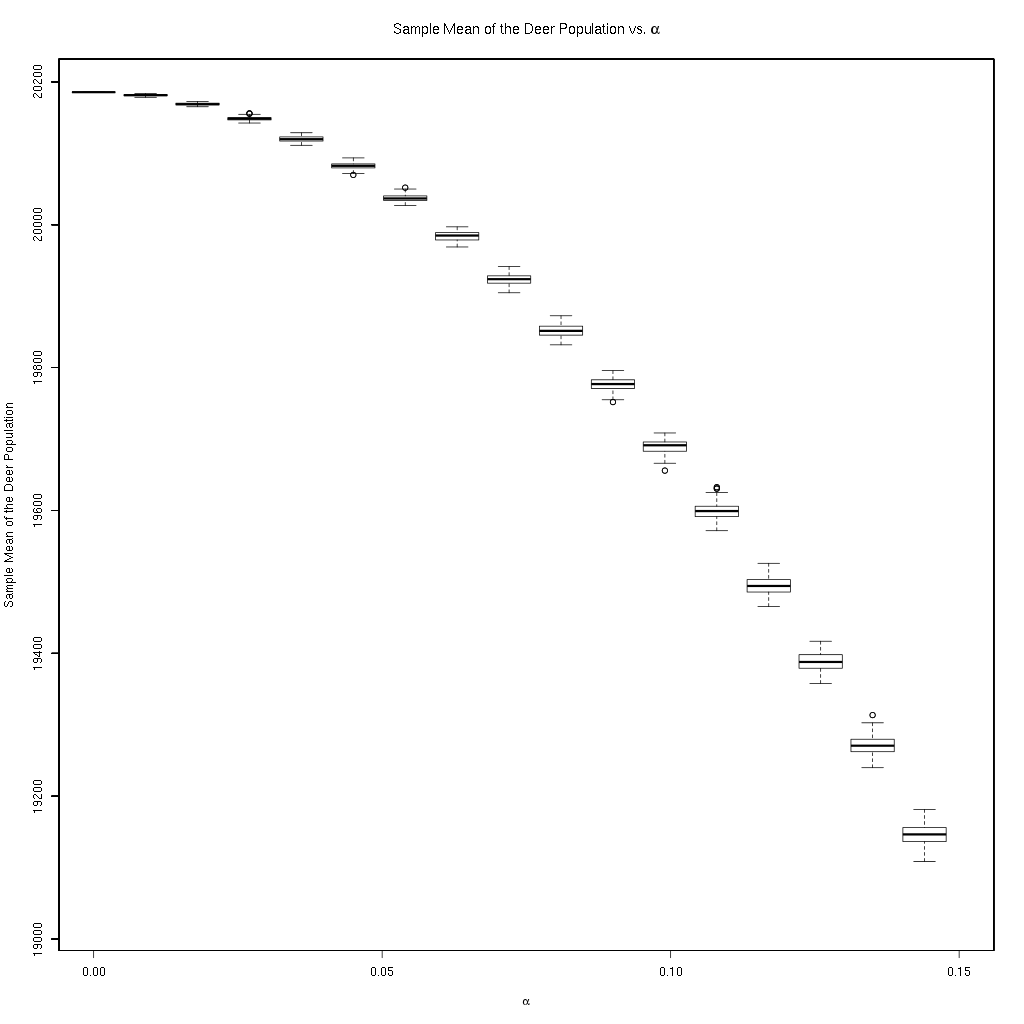
\includegraphics[width=5.2cm]{img/meanDeerByAlpha_boxplot}  
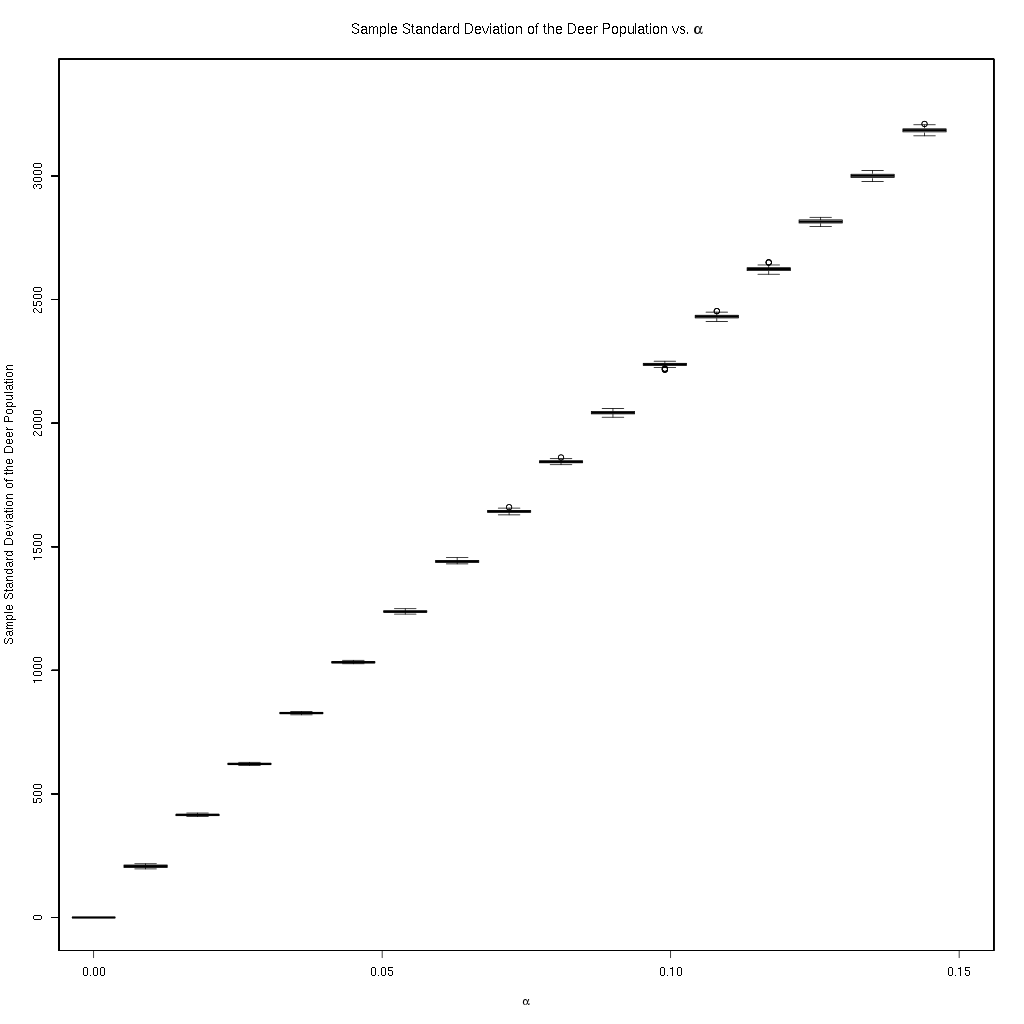
\includegraphics[width=5.2cm]{img/stdDevDeerbyAlpha_boxplot} \\
Boxplots of Sample Mean and Sample Standard Deviation of Deer Population \\
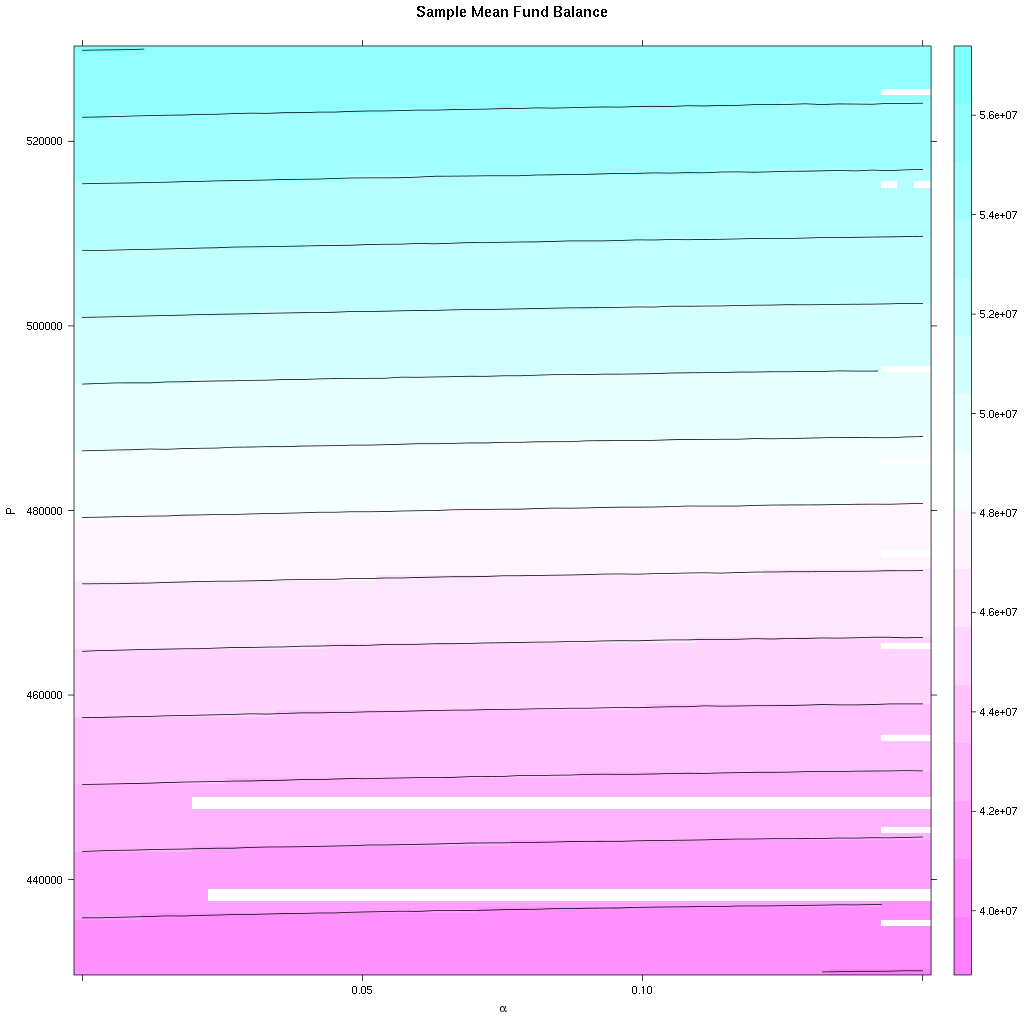
\includegraphics[width=5.25cm]{img/fundMeanContour} 
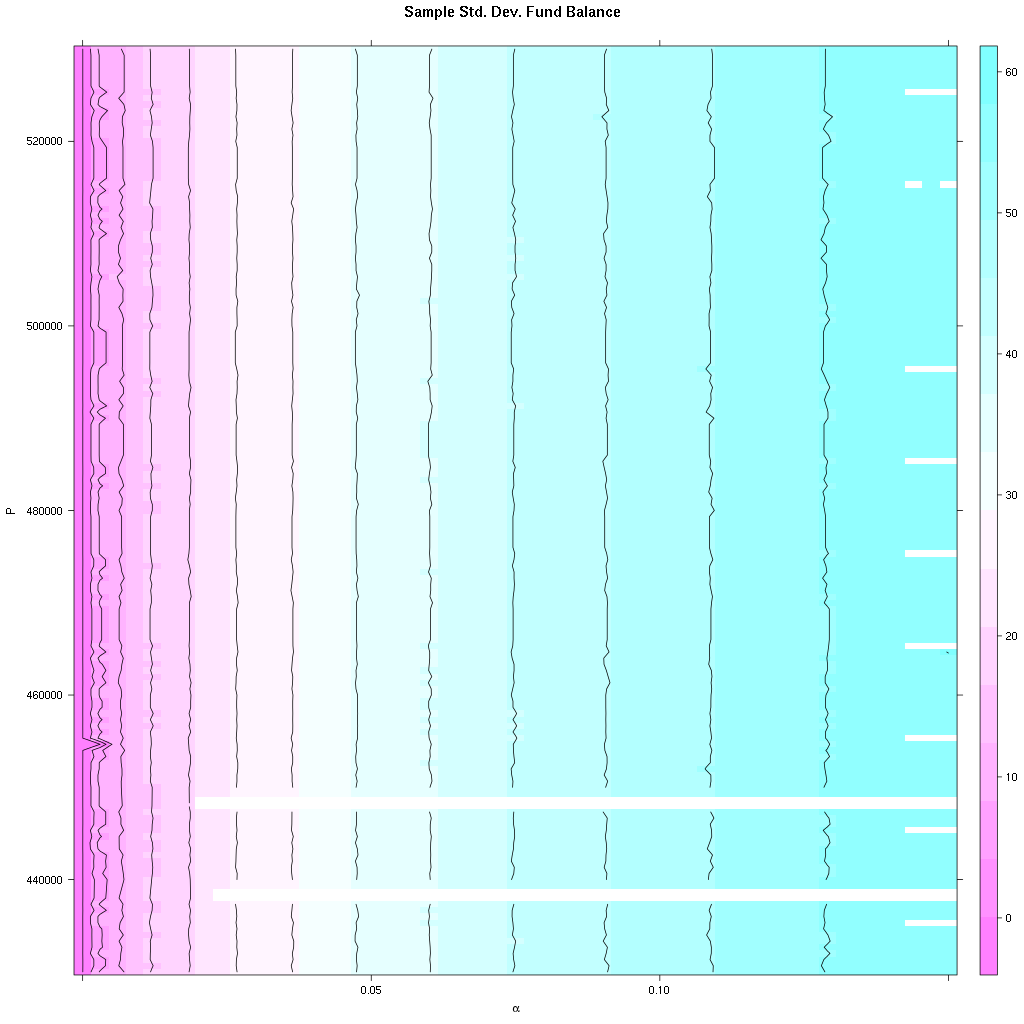
\includegraphics[width=5.25cm]{img/fundSDContour} \\
Contour Plots of Insurance Fund Balance \\
 }

%%%%%%%%%%%%%%%%%%%%%%%%%%%%%%%%%%%%%%%%%%%%%%%%%%%%%%%%%%%%%%%%%%%%%%%%%%%%%%
  \headerbox{Assumptions}{name=solve,column=0,below=definition,above=bottom}{
To identify a way of modeling the interaction of deer population and insurance funds, our assumptions for the model:
\begin{itemize}
	\item The population is near carrying capacity.
	\item The only predation is human i.e. hunting and car fatalities.
	\item Migration rates are balanced across counties.
	\item Customers of one insurance company experience the same collision rate as the general population.
\end{itemize}
}

%%%%%%%%%%%%%%%%%%%%%%%%%%%%%%%%%%%%%%%%%%%%%%%%%%%%%%%%%%%%%%%%%%%%%%%%%%%%%%
\headerbox{Stochastic Model}{name=history,column=1,below=simple}
{
By altering the scaled logisitic equation (\ref{eqn:scaled}) and including noise in the system, the stochastic model is \vspace*{-.4cm}
\begin{eqnarray}
dx &=& \tilde{r}x \left( 1- \frac{x}{\tilde{f}} \right) dt + \alpha x dW, \\
dm &=& (\rho m - \beta x + P)dt - \gamma x dW.
\end{eqnarray} \vspace{-.2cm}
The unknown parameters are
\begin{itemize}
	\item $\alpha$ - carrying capacity \vspace*{-.3cm}
	\item $\gamma$ - growth rate \vspace*{-.3cm}
	\item $P$ - harvest rate,
\end{itemize} \vspace*{-.2cm} and will be explored to see its impact on the interaction of deer population and insurance funds.
}

%%%%%%%%%%%%%%%%%%%%%%%%%%%%%%%%%%%%%%%%%%%%%%%%%%%%%%%%%%%%%%%%%%%%%%%%%%%%%%%
%\headerbox{Future Research}{name=app, column=3, below=graphs}{
%For the future, multivariate sensitivity should be examined and the initial value of $M$ could be explored as it could be a value that %is too big.
%}

%%%%%%%%%%%%%%%%%%%%%%%%%%%%%%%%%%%%%%%%%%%%%%%%%%%%%%%%%%%%%%%%%%%
\headerbox{Acknowledgments}{name=ref,column=3,above=bottom}{
Thanks to Dr. Foisy, Dr. Black, and NSF (NSF\# 1262737 for their involvement in this program and also to Anne Shelton and Brian Macherone from the
Research IT group at SUNY Albany for their support in
using their parallel computational facilities.
%\smaller
%\bibliographystyle{ieee}
%\renewcommand{\section}[2]{\vskip 0.05em}
%\begin{thebibliography}{1}\itemsep=-0.01em
%\setlength{\baselineskip}{0.4em}
%\bibitem{biology}
%\url{http://www.plosbiology.org/article/info}
%\bibitem{reproductive}
%\url{http://www.ganfyd.org/index.php?title=Reproductive_number}
%\end{thebibliography}
%\vspace{0.3em}
}


%%%%%%%%%%%%%%%%%%%%%%%%%%%%%%%%%%%%%%%%%%%%%%%%%%%%%%%%%%%%%%%%%%%
\headerbox{Conclusion}{name=infections,column=2,above=bottom}{
The stochastic model of deer population and insurance bond funds was consistent with the basic benchmarks. The model is most sensitive to $\alpha$. There is a linear relationship between $M$ and $P$. For the future, multivariate sensitivity should be examined as well as the initial value of $M$.
}
\end{poster}

\end{document}
